\part*{Modelo de Datos}

\section{Variables Aleatorias}

\begin{itemize}
    \item[A)] Cantidad de proyectos por mes
    \item[B)] Tipo de proyecto
    \item[C)] Tamaño de proyecto [h]
    \item[D)] Precio hora-hombre del proyecto [\$]
    \item[E)] Plazo de entrega del proyecto [h]
\end{itemize}

\section{Estrategia de obtención}

Para obtener las distribuciones de las variables aleatorias que utilizará el simulador, se tomaron muestras de los proyectos de algunas software factories. Luego se 
adaptaron a las distribuciones conocidas más similares, para simplificar el análisis y desarrollo del simulador. Los datos corresponden a los últimos 2 años. \\

A continuación se detallan las distribuciones de las distintas variables aleatorias.\\

\section*{Llegada de proyectos}
Para la generación de esta variable aleatoria se decidió utilizar una distribución de Poisson con media ($\lambda$) 3. Se considera que esto aproxima correctamente
la realidad. \\

\begin{figure}[H]
\begin{center}
 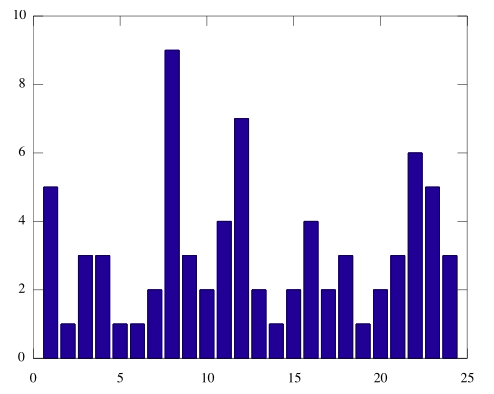
\includegraphics[width=0.75\textwidth,height=0.75\textheight,keepaspectratio]{./images/projects-arrivals.png}
 % projects-arrivals.png: 1200x900 pixel, 150dpi, 20.32x15.24 cm, bb=0 0 576 432
\end{center}
\caption{Gráfico de barras correspondiente a la llegada de proyectos.}
\end{figure}

\section*{Tipo de proyecto}

Para la variable aleatoria de tipo de proyecto, se estableció el uso de una distribución uniforme con las siguientes proporciones: 

\begin{itemize*}
    \item Grande: 15\%
    \item Mediano: 75\%
    \item Pequeño: 10\%
\end{itemize*}

\begin{figure}[H]
\begin{center}
 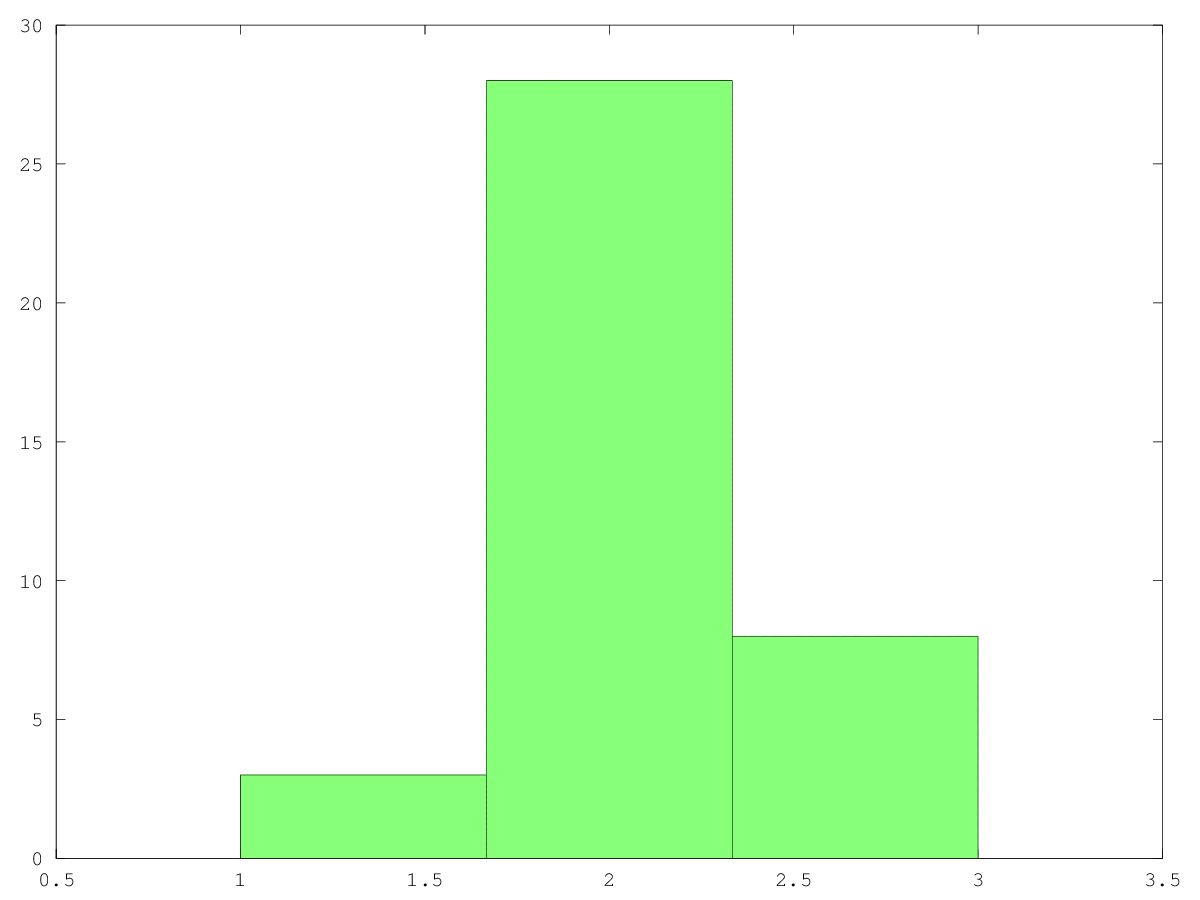
\includegraphics[width=0.75\textwidth,height=0.75\textheight,keepaspectratio]{./images/proyect-types.png}
 % proyect-types.png: 1200x900 pixel, 150dpi, 20.32x15.24 cm, bb=0 0 576 432
\end{center}
\caption{Histograma de los tipos de proyectos. El 1 representa un tamaño pequeño, el 2 mediano y el 3 grande.}
\end{figure}

\section*{Horas Hombre de proyecto}

Dado que no se contaba con un gran número de muestras, y las distribuciones no podían ser fácilmente distinguidas, o no parecían seguir fielmente ninguna de las distribuciones
más conocidas, se utilizó una distribución triangular, para aproximar según alguna ``buena estimación''. Por esto, para la generación de la variable aleatoria se utilizó, 
según el tipo de proyecto sea pequeño, mediano o grande, una distribución triangular con parámetros (500, 2000, 1400), (2000, 4500, 3200) y (4500, 8000, 5300).

\begin{figure}[H]
\begin{center}
 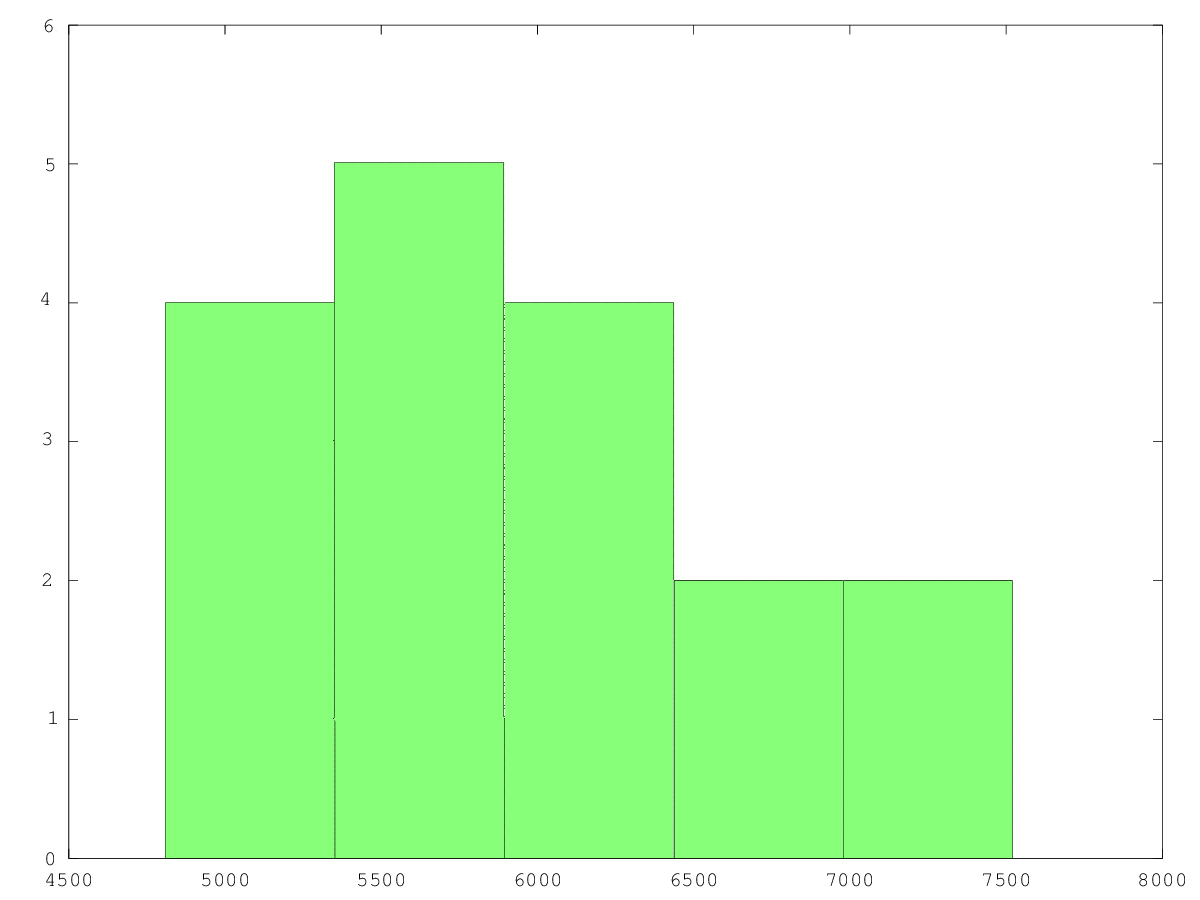
\includegraphics[width=0.75\textwidth,height=0.75\textheight,keepaspectratio]{./images/data-big-hours.png}
 % data-big-hours.png: 1200x900 pixel, 150dpi, 20.32x15.24 cm, bb=0 0 576 432
\end{center}
\caption{Histograma de las horas hombre de proyecto, para proyectos de tamaño grande.}
\end{figure}

\begin{figure}[H]
\begin{center}
 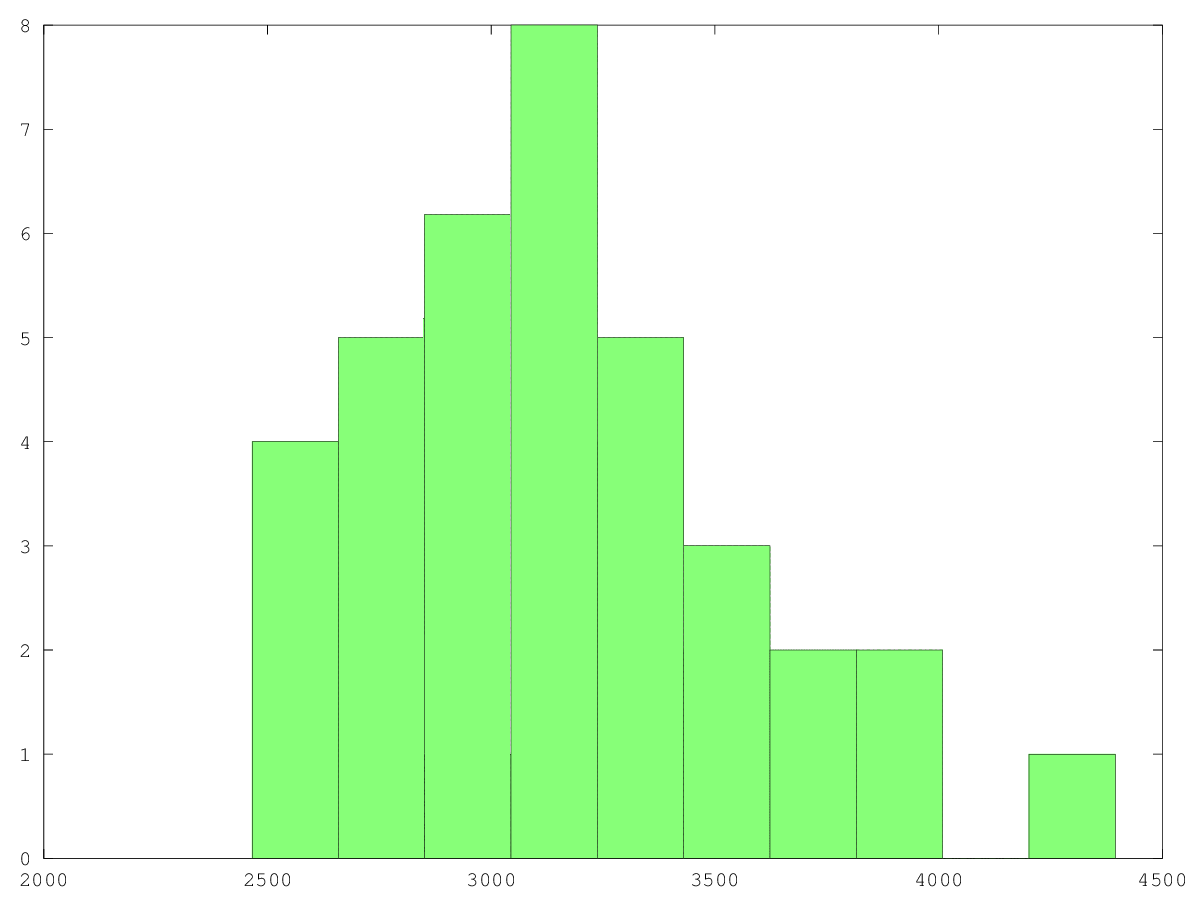
\includegraphics[width=0.75\textwidth,height=0.75\textheight,keepaspectratio]{./images/data-medium-hours.png}
 % data-medium-hours.png: 1200x900 pixel, 150dpi, 20.32x15.24 cm, bb=0 0 576 432
\end{center}
\caption{Histograma de las horas hombre de proyecto, para proyectos de tamaño mediano.}
\end{figure}

\begin{figure}[H]
\begin{center}
 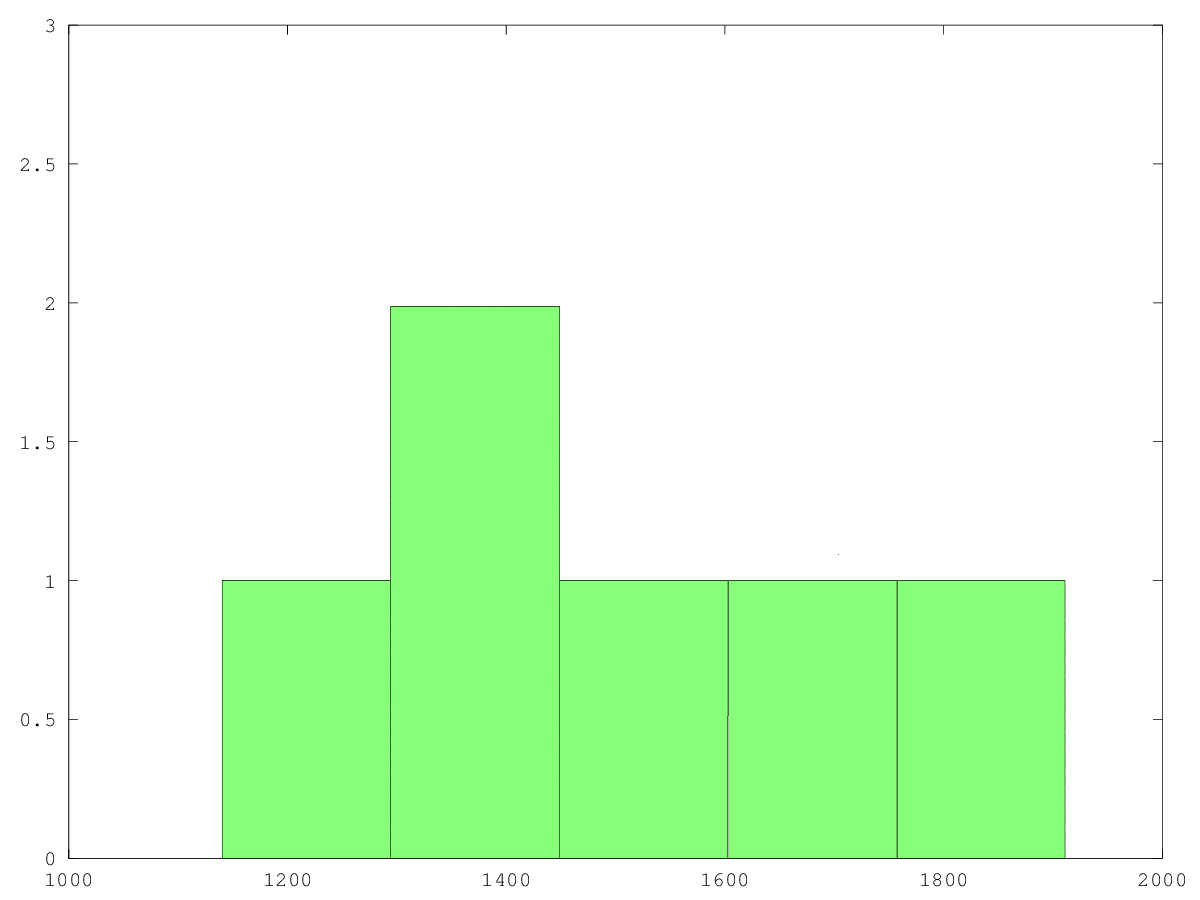
\includegraphics[width=0.75\textwidth,height=0.75\textheight,keepaspectratio]{./images/data-small-hours.png}
 % data-small-hours.png: 1200x900 pixel, 150dpi, 20.32x15.24 cm, bb=0 0 576 432
\end{center}

\caption{Histograma de las horas hombre de proyecto, para proyectos de tamaño pequeño.}
\end{figure}

\section*{Precio por hora de proyecto}
De nuevo, como se contaba con una gran cantidad de muestras, se utilizaron distribuciones triangulares para intentar aproximar dados algunos criterios estimativos. Para la generación 
de esta variable aleatoria se utilizó entonces una distribución triangular, variando sus parámetros según el tamaño del proyecto fuese pequeño, mediano o grande. Los valores de estos
parámetros fueron (200, 310,290), (200, 240, 220) y (180, 310, 230), respectivamente.

\begin{figure}[H]
\begin{center}
 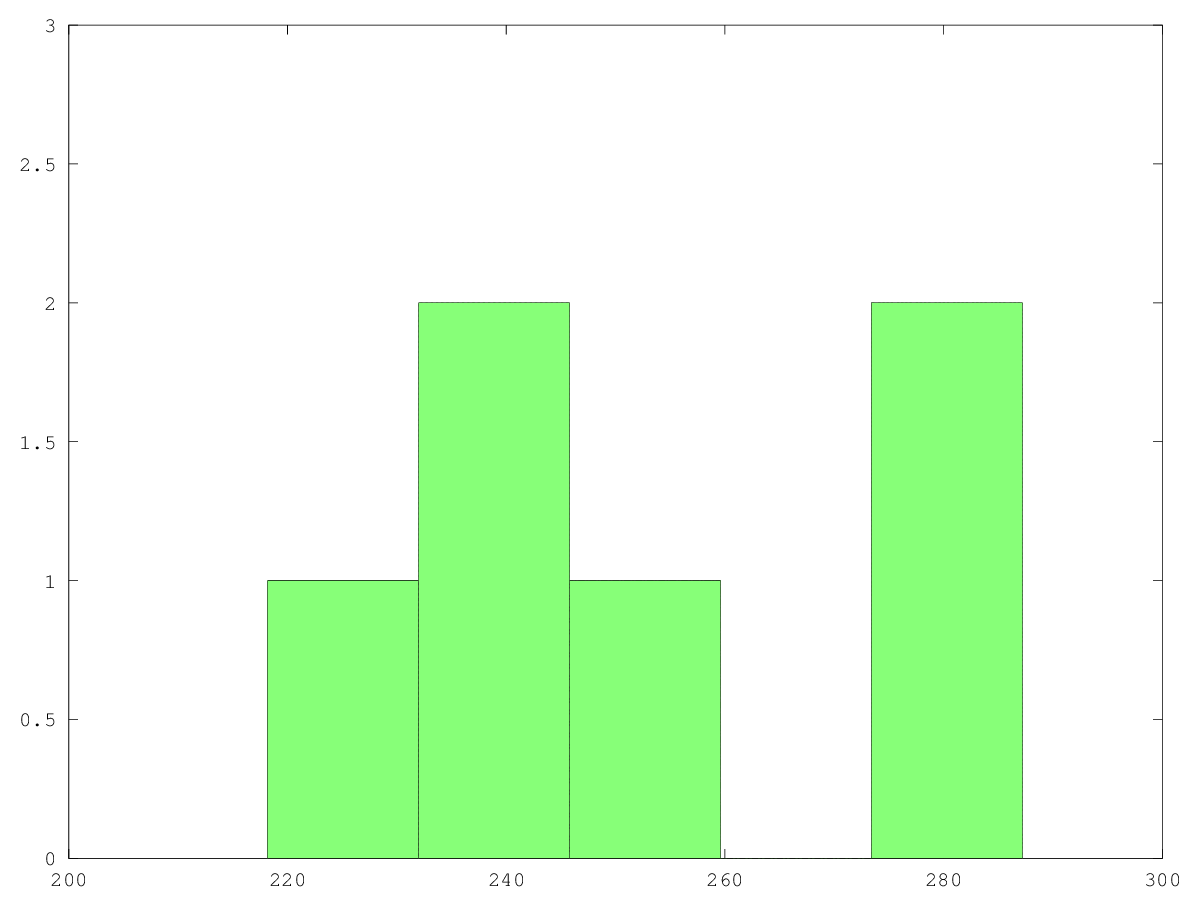
\includegraphics[width=0.75\textwidth,height=0.75\textheight,keepaspectratio]{./images/data-big-money.png}
 % data-big-money.png: 1200x900 pixel, 150dpi, 20.32x15.24 cm, bb=0 0 576 432
\end{center}
\caption{Histograma de precio por hora de proyecto, para proyectos de tamaño grande.}
\end{figure}


\begin{figure}[H]
\begin{center}
 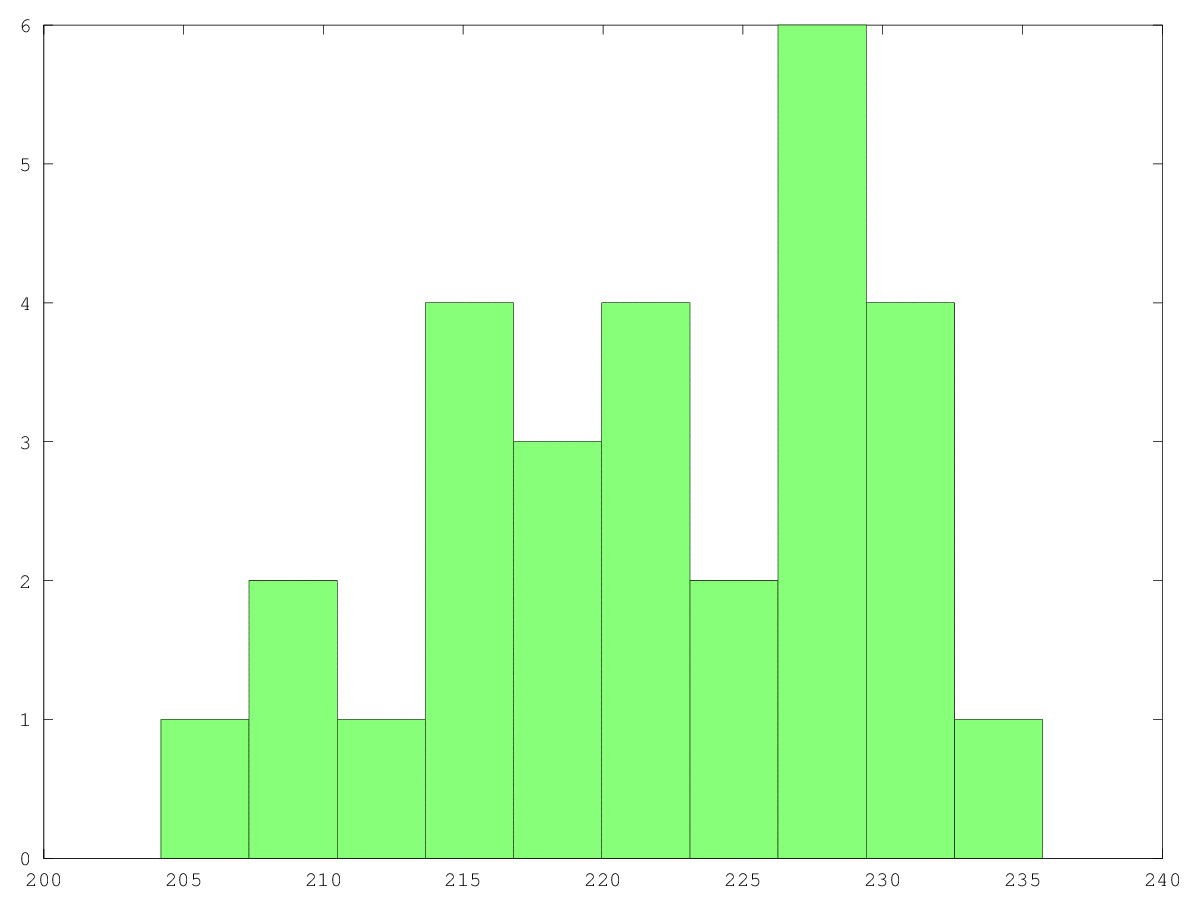
\includegraphics[width=0.75\textwidth,height=0.75\textheight,keepaspectratio]{./images/data-medium-money.png}
 % data-medium-money.png: 1200x900 pixel, 150dpi, 20.32x15.24 cm, bb=0 0 576 432
\end{center}
\caption{Histograma de precio por hora de proyecto, para proyectos de tamaño mediano.}
\end{figure}

\begin{figure}[H]
\begin{center}
 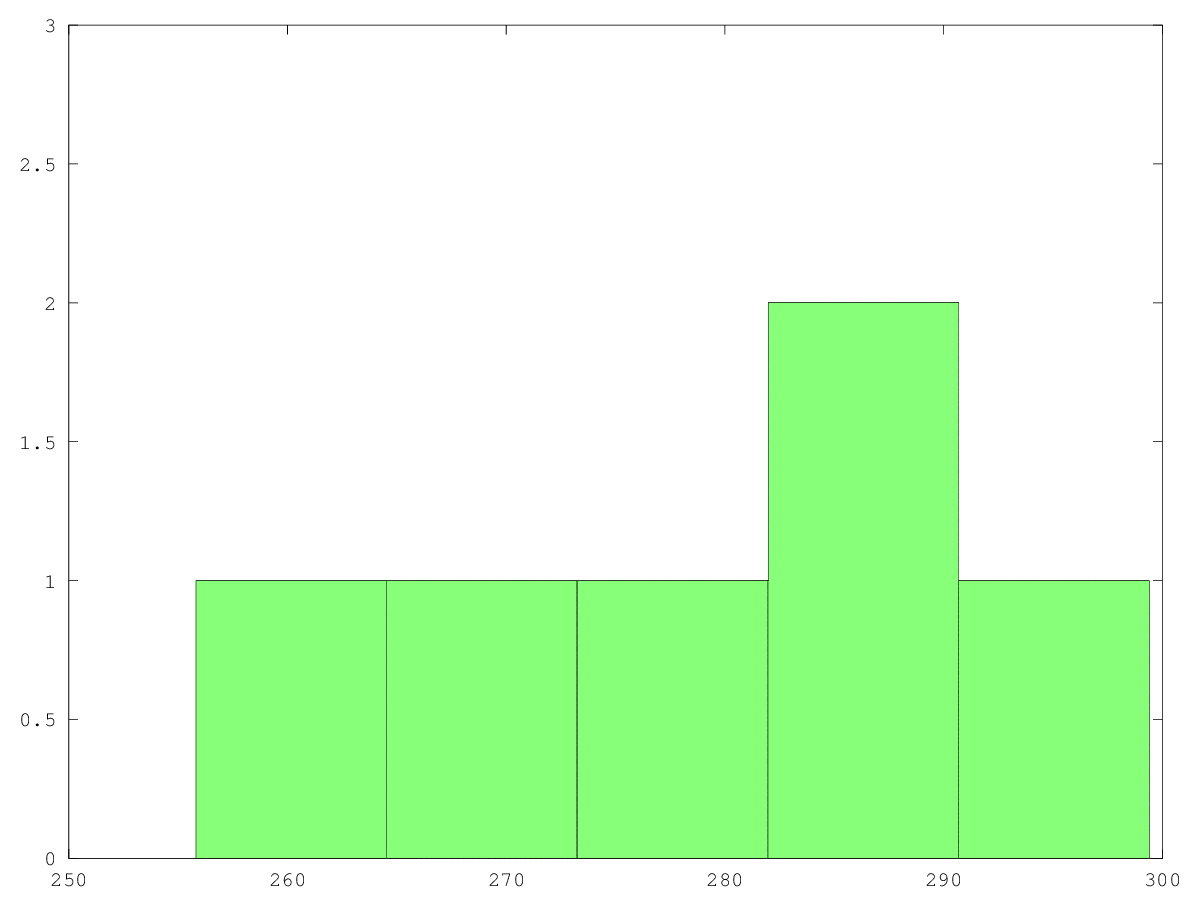
\includegraphics[width=0.75\textwidth,height=0.75\textheight,keepaspectratio]{./images/data-small-money.png}
 % data-small-money.png: 1200x900 pixel, 150dpi, 20.32x15.24 cm, bb=0 0 576 432
\end{center}
\caption{Histograma de precio por hora de proyecto, para proyectos de tamaño pequeño.}
\end{figure}

\section*{Fecha de entrega de proyecto}

Para la generación de esta variable aleatoria, dada su complejidad, se buscó relacionarla con la variable aleatoria de las horas hombre de un proyeco y la cantidad de desarrolladores
promedio que se asignan a cada tipo de proyecto (pequeño, mediano o grande). El resultado fue la utilización de una distribución triangular, cuyo parámetros se definieron de la siguiente 
forma:

\begin{itemize*}
    \item[($a$)] el mínimo de la distribución se forma tomando el valor de la variable Horas Hombre y diviéndolo por el \textit{máximo} de la cantidad de desarrolladores que en promedio
    se le asignan a ese tipo de proyecto.
    \item[($b$)] el máximo de la distribución surge de la división entre el valor de la variable Horas Hombre y el \textit{mínimo} de la cantidad de desarrolladores que en promedio
    se le asignan a ese tipo de proyecto.
    \item[($c$)] la moda de la distribución se calcula, de la misma forma, diviéndo el valor de la variable Horas Hombre por la \textit{moda} de la cantidad de desarrolladores que en promedio
    se le asignan a ese tipo de proyecto.
\end{itemize*}
 

\section*{Tabla de valores}

A continuación se presentan los resultados de esta sección resumidos en 2 tablas de valores, con los parámetros de cada distribución.\\

\begin{table}[H]
\begin{center}
\begin{tabular}{|l|c|}
\hline
    Tipo        & Porcentaje\\
\hline
    Grande      & 15\%\\
\hline
    Mediano     & 75\%\\
\hline
    Pequeño     & 10\%\\
\hline
\end{tabular}

\end{center}

\caption{Cuadro de porcentajes de tipos de proyectos}
\label{tab:tipo-proyecto}

\end{table}

\begin{table}[H]

\begin{center}

\begin{tabular}{|l|l|l|l|l|}
\hline
                    & Tipo      & Mín.    & Máx.    & Moda\\
\hline
    Horas           & Grande    & 4500    & 8000    & 5300\\
\hline
                    & Mediano   & 2000    & 4500    & 3200\\
\hline
                    & Pequeño   & 500     & 2000    & 3200\\
\hline
    Precio          & Grande    & 180     & 310     & 230\\
\hline
                    & Mediano   & 200     & 240     & 220\\
\hline
                    & Pequeño   & 200     & 300     & 290\\
\hline
    Fecha de Entrega& Grande    & Horas/6 & Horas/4 & Horas/5\\
\hline
                    & Mediano   & Horas/4 & Horas/2 & Horas/3\\
\hline
                    & Pequeño   & Horas/3 & Horas/1 & Horas/2\\
\hline
\end{tabular}

\end{center}

\caption{Cuadro de valores para las distribuciones según tipo de proyecto}
\label{tab:va}


\end{table}

